%% =============================================================
%%  figures/placeholder.tex
%%
%%  This file contains no compiled content and is NOT \input anywhere
%%  in the thesis. It documents the naming and usage convention for
%%  the figures/ directory.
%% =============================================================

%% -------------------------------------------------------------
%% FOLDER CONVENTION
%% -------------------------------------------------------------
%% All figure source files (vector and raster) are stored flat in the
%% figures/ directory. main.tex sets \graphicspath{{figures/}}, so
%% every \includegraphics call in the chapter files should reference
%% only the filename (no path, no extension), e.g.:
%%
%%     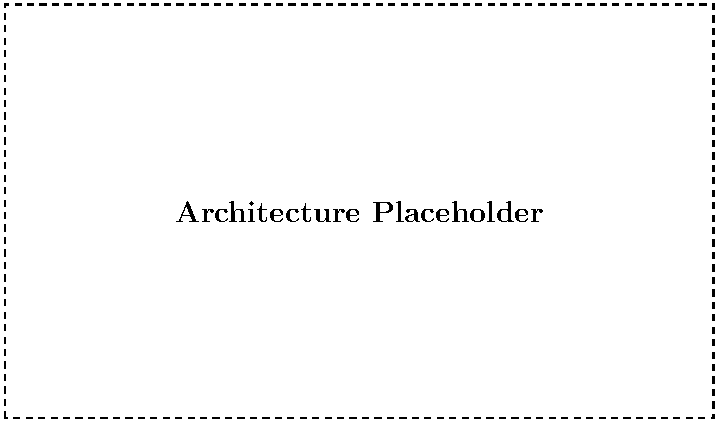
\includegraphics[width=0.85\textwidth]{system_architecture}
%%
%% and LaTeX will resolve system_architecture.pdf or .png automatically
%% from within figures/.

%% -------------------------------------------------------------
%% FILE NAMING
%% -------------------------------------------------------------
%% Use lowercase, underscore-separated, descriptive names that match
%% the figure's \label, e.g.:
%%   figures/system_architecture.pdf      -> \label{fig:system-architecture}
%%   figures/preprocessing_pipeline.pdf   -> \label{fig:preprocessing-pipeline}
%%   figures/classification_confusion_matrix.png -> \label{fig:classification-confusion}

%% -------------------------------------------------------------
%% FORMAT GUIDANCE
%% -------------------------------------------------------------
%% - Use PDF (vector) for diagrams, plots generated from data, and any
%%   figure that should remain crisp at any zoom level (block diagrams,
%%   architecture diagrams, line/bar charts). Export directly to PDF
%%   from the source tool (e.g. draw.io, matplotlib with plt.savefig
%%   using a .pdf extension, Inkscape).
%% - Use PNG (raster) only for photographs, camera frame screenshots,
%%   or renderings where vector export is not applicable. Use a
%%   resolution of at least 300 DPI at the intended print size.
%% - Avoid JPEG for anything containing text or sharp edges, since
%%   compression artefacts become visible when printed.

%% -------------------------------------------------------------
%% REFERENCING FIGURES IN TEXT
%% -------------------------------------------------------------
%% Every figure must be given a \label{fig:xxx} inside its figure
%% environment, and referenced at least once in the surrounding text
%% using \ref{fig:xxx} (or \Cref{fig:xxx} / \cref{fig:xxx} via the
%% cleveref package loaded in preamble.tex), e.g.:
%%
%%   \begin{figure}[H]
%%     \centering
%%     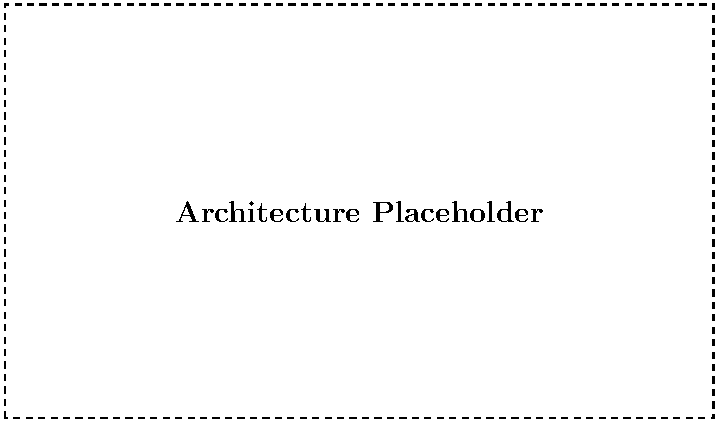
\includegraphics[width=0.85\textwidth]{system_architecture}
%%     \caption{Block diagram of the proposed system architecture.}
%%     \label{fig:system-architecture}
%%   \end{figure}
%%
%%   As shown in Figure~\ref{fig:system-architecture}, ...
%%
%% Never reference a figure by a hard-coded number -- always use
%% \ref or \Cref so that numbering stays correct if chapters/figures
%% are reordered.

%% -------------------------------------------------------------
%% CURRENT PLACEHOLDER FIGURES REFERENCED BY THE CHAPTER FILES
%% -------------------------------------------------------------
%% The following figure files are referenced by \includegraphics calls
%% in the chapter files but do not yet exist on disk. pdflatex will
%% report "file not found" warnings for these until the real figures
%% are added to this directory:
%%
%%   figures/system_architecture.pdf        (Chapter 4)
%%   figures/preprocessing_pipeline.pdf      (Chapter 6)
%%   figures/classification_confusion_matrix.png (Chapter 8)
%%   figures/pose_qualitative_results.png    (Chapter 8)
%%
%% %% TODO: Create/export each of the above figures and place them in
%% this directory using the naming convention described above.
